\begin{homeworkProblem}
Three identical atoms at the corner of  an equilateral triangle can be considered as  a graphen unite cell. Assume that each atom contributes one electron. By neglecting electron -electron interaction Matrix representation of the Hamiltonian for each electron in the localized basis is:
\begin{equation}
\A{H}_0=
\begin{pmatrix}
E_0 & -a &-a\\
-a&E_0&-a\\
-a&-a&E_0
\end{pmatrix}
\end{equation}
where $E_0$ is the self energy of the electron shared by each atom. $a$ describes nondiagonal terms originateing form adjacent site wave function overlap. In this repersenation expanding basis functions which are designated by $\ket{1}$ , $\ket{2}$ and $\ket{3}$ are the sates vectors describing each atom at its own site. 


\begin{homeworkSection}{(a)}

To calculate energy eigenvalues of the system we have to solve the following eigen value problem:
\begin{equation}
\A{H}_0\vp{\Psi}=E\vp{\Psi}\quad\Lrw\quad 
\begin{pmatrix}
E_0 & -a &-a\\
-a&E_0&-a\\
-a&-a&E_0
\end{pmatrix}
\begin{pmatrix}
\psi_1\\
\psi_2\\
\psi_3
\end{pmatrix}
=E\begin{pmatrix}
\psi_1\\
\psi_2\\
\psi_3
\end{pmatrix}
\end{equation}
where $\vp{\Psi}$ is the matrix representation (isomorophism) of the state 
$$\ket{\Psi}=\psi_1\ket{1}+\psi_2\ket{2}+\psi_3\ket{3}$$
So we have:
\begin{equation}
\det
\begin{pmatrix}
E_0-E & -a &-a\\
-a&E_0-E&-a\\
-a&-a&E_0-E
\end{pmatrix}
=0
\quad\Lrw\quad
\left\{
\begin{array}{l}
E_1=E_0-2a\\
E_2=E_0+a\\
E_3=E_0+a
\end{array}
\right.
\end{equation}
$E_1$ , $E_2$ and $E_3$ are three energy eigenvalues. $E_1$ corresponds to the ground state of the system. As we can see $E_2=E_3$ so there is a two-fold degeneracy  in this eigen vlue problem.
 The associated eigenvectors are:

\begin{equation}
E=E_1\quad \Lrw\quad 
\begin{pmatrix}
2a  & -a &-a\\
-a& 2a &-a\\
-a&-a& 2a
\end{pmatrix}
\begin{pmatrix}
\psi_1\\
\psi_2\\
\psi_3
\end{pmatrix}
=0
\quad\Lrw\quad
\vp{\Psi}_1=
\frac{1}{\sqrt{3}}
\begin{pmatrix}
1\\
1\\
1
\end{pmatrix}
\end{equation}
Since two other eigenvalues are degenerate we have a kind of freedome in selecting two other eigenstates. As a mater of the fact we have to just find two orthonormal vectors which both lie in $\psi_1+\psi_2+\psi_3=0$ plane:
\begin{equation}
E=E_2,E_3\quad \Lrw\quad 
\begin{pmatrix}
-a  & -a &-a\\
-a& -a &-a\\
-a&-a& -a
\end{pmatrix}
\begin{pmatrix}
\psi_1\\
\psi_2\\
\psi_3
\end{pmatrix}
=0
\quad\Lrw\quad
\psi_1+\psi_2+\psi_3=0
\end{equation}
 we just choose:
 \begin{equation}
 \vp{\Psi}_2=
 \frac{1}{\sqrt{2}}
 \begin{pmatrix}
1\\
-1\\
0
\end{pmatrix}
\qquad
\vp{\Psi}_3=
 \frac{1}{\sqrt{6}}
 \begin{pmatrix}
1\\
1\\
-2
\end{pmatrix}
 \end{equation}
 Since now $\ket{\Psi_1}$, $\ket{\Psi_2}$ and $\ket{\Psi_3}$ are abstract state kets correspond to $\vp{\Psi}_1$ , $\vp{\Psi}_2$ and $\vp{\Psi}_3$ respectively. 

\end{homeworkSection}
%---------b------------
\begin{homeworkSection}{(b)}
Suppose a static electrical field is applied to the system such that potential energy of the electron on the top of the triangle is lowered by $V_0$ which is assumed it's so smaller than $a$. Actually this electrial field purturbs the Hamiltonian. From the primary assumptions we have:
\begin{equation}\label{P5-look}
\A{H}=\A{H}_0+\gamma\A{H}_1=
\begin{pmatrix}
E_0-V_0 & -a &-a\\
-a & E_0 &-a \\
-a &-a &-E_0
\end{pmatrix}
\end{equation}
where $\gamma$ is dimensionless parameter and is defined as
\begin{equation}
\gamma=\frac{V_0}{a}
\end{equation}
and $H_1$ is the purturbing Hamiltonian 
\begin{equation}
\A{H}_1=
\begin{pmatrix}
-a & 0 & 0\\
0 & 0 & 0\\
0 & 0 & 0
\end{pmatrix}
\end{equation}
To evaluate the new energy eigenvalues and associated eigenstates the direct diagonalization procedure is given at first and then  the general formulation of \textit{time independent purturbation theory} is applied to give a better insight about energy shift and break of degeneracy.

In order to diagonolize the new Hamiltonian the follwoing eigenvalue problem should be solved:
\begin{equation}
H\ket{\Psi}=\lambda\ket{\Psi}
\end{equation} 
If we take a look at matrix representation of $H$ it can be seen that $H$ can be rewritten as below:
\begin{equation}\label{P5-1}
\A{H}=E_0\vp{I}_{3\times 3}-a
\begin{pmatrix}
\gamma & 1 &1\\
1&0& 1\\
1&1&0
\end{pmatrix}
\end{equation}
where $\vp{I}_{3\times 3}$ is $3\time 3$ unity matrix.
 for every eigenvalue we have $\lambda=E_0-a\lambda_1$ where $\lambda_1$ is eigenvalue of the second matrix in the right hand side of \eqref{P5-1}. So we have to just work on the second matrix. 
 \begin{equation}
 \det
 \begin{pmatrix}
\gamma-\lambda_1 & 1 &1\\
1&-\lambda_1 & 1\\
1 & 1 & -\lambda_1
\end{pmatrix}
=0
\quad\Lrw\quad
(\gamma-\lambda_1)(\lambda_1^2-1)+2(\lambda_1+1)=0
 \end{equation}
Note that since $V_0\ll a$ then $\gamma\ll 1$. Therefore:
\begin{equation}
\left\{
\begin{array}{lcl}
\lambda_1=\frac{1+\gamma}{2}+\sqrt{\frac{(1+\gamma)^2}{4}+2-\gamma}&\Lrw & E_1\approx E_0-a\left(2+\frac{\gamma}{3}\right)=E_0-2a-\frac{1}{3}V_0\\
\lambda_1=\frac{1+\gamma}{2}-\sqrt{\frac{(1+\gamma)^2}{4}+2-\gamma}&\Lrw & E_2\approx E_0-a\left(-1+\frac{2}{3}\gamma\right)=E_0+a-\frac{2}{3}V_0\\
\lambda_1=1 &\Lrw& E_3=E_0+a
\end{array}
\right.
\end{equation}
First order approximation  has been applied  to get the final results. Applied electrical fiels breaks the symmetry and removes the degeneracy. The formulation of the problem based on time independent perturbation theory is developed in continue. 

Let us assume that we have found the eigen value and the complete set of normalized eigenfunctions for a Hamiltonian $H_0$,
\begin{equation}
H_0\ket{\Psi_n}=E_n^{(0)}\ket{\Psi_n}
\end{equation}
We now ask to solve
\begin{equation}\label{P5-10}
\left(H_0+\gamma H_1\right)\ket{\Phi_n}=E_n\ket{\Phi_n}
\end{equation}
In general we may view the Hamiltonian as a matrix, we can write:
\begin{equation}
\A{H}_{mn}=\bra{\Psi_m}H\ket{\Psi_n}=E_{m}^{(0)}\delta_{mn}+\bra{\Psi_m}\gamma H_1\ket{\Psi_n}
\end{equation}
We will express the desired quantities as a power series in $\gamma$. and we will assume that as $\gamma\rightarrow 0$,
$E_n\rightarrow E_n^{(0)}$.

Since $\ket{\Psi_n}$ form a complete set, we may expand $\ket{\Phi_n}$ in series invoving $\ket{\Psi_n}$ ,
\begin{equation}
\ket{\Phi_n}=N(\gamma)\left\{\ket{\Psi_n}+\sum_{k\neq n}C_{nk}(\gamma)\ket{\Psi_n}\right\}
\end{equation}
The factor $N(\gamma)$ is the normalization coefficient guarating  $\bracket{\Phi_n}{\Phi_n}=1$. Note that if $\gamma=0$ then we should have:
\begin{equation}
N(0)=1\qquad C_{nk}(0)=0\qquad E_{n}(0)=E_n^{(0)}
\end{equation}
This allows us to expance $C_{nk}(\gamma)$  and $E_n(\gamma)$ as a power series of $\gamma$ :
\begin{align}
C_{nk}(\gamma) &=\gamma C_{nk}^{(1)}+\gamma^2 C_{nk}^{(2)}+\cdots\label{P5-Cexp}\\
E_{n}(\gamma)&=E_n^{(0)}+\gamma E_n^{(1)}+\gamma^2 E_n^{(2)}+\cdots\label{P5-Eexp}
\end{align}
Insering \eqref{P5-Cexp} and \eqref{P5-Eexp} into \eqref{P5-10} leads to a set of equations. Identifying powers of $\gamma$  yields a seris of equations. The first one is:
\begin{equation}\label{P5-100}
H_0\sum_{k\neq n}C_{nk}^{(1)}\ket{\Psi_k}+H_1\ket{\Psi_n}=E_n^{(0)}\sum_{k\neq n}C_{nk}^{(1)}\ket{\Psi_k}+E_n^{(1)}\ket{\Psi_n}
\end{equation}
Mutiplying both sides of \eqref{P5-100} by $\bra{\Psi_n}$ and using orthogonality condition we obtain
\begin{equation}\label{P5-energyshift}
\gamma E_n^{(1)}=\bra{\Psi_n}\gamma H_1\ket{\Psi_n}
\end{equation}
This showes the first order energy shift in the energy levels. Similarly if we multiply both sides of \eqref{P5-100} by $\bra{\Psi_m}$ we obtain:
\begin{equation}\label{P5-Cnm}
\gamma C_{nm}=\frac{\bra{\Psi_m}\gamama H_1\ket{\Psi_n}}{E_n^{(0)}-E_m^{(0)}}
\end{equation}
\end{homeworkSection}
The numerator is the matrix elements of $\gamma H_1$ in basis of states in which $H_0$ is diagonal. First order energy shift and the coefficients of the other basis expanding new eigenstates of the purturbed Hamiltonian were given. In deriving \eqref{P5-Cnm} it's assumed that there is no  degeneracy i.e. $E^{(0)}_n\neq E^{(0)}_k $ for $k\neq n$.  Quite generally  assume a subspace made of some orthogonal eigen states of original Hamiltonian is a degenerates subspace ,i.e. the the expecation value of the original Hamiltonian evaluated on every state vector in this subspace is constant. Suppose that an unitary operator acts only on this subsapce and rotates orthogonal basis functions. Defenitely Hamiltonian in the rotated states is still diagonal. Now we can rotate the subspace to digonalize $\gamma H_1$ without affecting the states out side of this subspace. In this case digonalized purturbing Hamiltonian directly shifts energy levels in the first order . Cleraly diagonalizing $H_1$ in the degenerate subspace leads to the determination of proper eigen states.  

Now we can apply this theory to our original problem. First we can readily evaluate the first order (in term of $\gamma$) energy shift for the ground state. Since the ground state is not a degenerate state we can use ordinary perturbation theory. From \eqref{P5-energyshift} we have:
\begin{equation}
\gamma E_1^{(1)}=\bra{\Psi_1}\gamma H_1\ket{\Psi_1}=\gamma\vp{\Psi}_1^\dagger \A{H}\vp{\Psi}_1=\frac{-V_0}{3}\left(\bra{1}+\bra{2}+\bra{3}\right)\ket{1}\bra{1}\left(\ket{1}+\ket{2}+\ket{3}\right)=-\frac{V_0}{3}
\end{equation}
If we use \eqref{P5-Cnm} then:
\begin{align}
&\gamma C_{12}=\gamma\frac{\vp{\Psi}_2^\dagger\A{H}_1\vp{\Psi}_1}{(E_0-2a)-(E_0+a)}=
-\frac{\gamma}{3\sqrt{6}}\\
&\gamma C_{13}=\gamma\frac{\vp{\Psi}_3^\dagger\A{H}_1\vp{\Psi}_1}{(E_0-2a)-(E_0+a)}=
-\frac{\gamma}{9\sqrt{2}}
\end{align}
So we have:
\begin{equation}\label{P5-ground}
c\ket{\Phi_1}=\left(1-\frac{2\gamma}{9}\right)\ket{1}+\left(1+\frac{\gamma}{9}\right)\ket{2}+\left(1+\frac{\gamma}{9}\right)\ket{3}
\end{equation}
To evaluate energy shift in the degenerate states we should first reprsent $H_1$ in $\ket{\Psi_i}$ basis:
\begin{equation}
\A{H}'_1=-V_0
\begin{pmatrix}
\frac{1}{3} & \frac{1}{\sqrt{6}} &\frac{1}{3\sqrt{2}}\\
\frac{1}{\sqrt{6}} & \frac{1}{2} & \frac{1}{2\sqrt{3}}\\
\frac{1}{2\sqrt{2}} & \frac{1}{2\sqrt{3}} & \frac{1}{6}
\end{pmatrix}
\end{equation}

At this stage we should digonalize the $2\time 2$ bloch matrix the lower corner of $\A{H}'_1$:
\begin{equation}
-V_0
\begin{pmatrix}
 \frac{1}{2} & \frac{1}{2\sqrt{3}}\\
 \frac{1}{2\sqrt{3}} & \frac{1}{6}
\end{pmatrix}\vp{\Phi}'
=\lambda \vp{\Phi}'\quad\Lrw\quad 
\left\{
\begin{array}{ll}
\lambda=0 & \vp{\Phi}'_2=\frac{1}{2}\left(1\quad -\sqrt{3}\right)^T\\
\lambda=-\frac{2V_0}{3}& \vp{\Phi}'_3=\frac{1}{2}\left(\sqrt{3}\quad 1\right)^T\\
\end{array}
\right.
\end{equation}
New eigenstates can be reprsented in the old basis as:

\begin{align}
&\ket{\Phi_2}=\frac{1}{2}\ket{\Psi_2}-\frac{\sqrt{3}}{2}\ket{\Psi_3}=-\frac{1}{\sqrt{2}}\ket{2}+\frac{1}{\sqrt{2}}\ket{3}\\
&\ket{\Phi_3}=\frac{\sqrt{3}}{2}\ket{\Psi_2}+\frac{1}{2}\ket{\Psi_3}=\sqrt{\frac{2}{3}}\ket{1}-\frac{1}{\sqrt{6}}\ket{2}+\frac{1}{\sqrt{6}}\ket{3}
\end{align}

The result of our analysis is shown in the figure \ref{fig-P5}.
\begin{figure}[h]
\centering
% Generated with LaTeXDraw 2.0.8
% Fri Feb 15 20:32:27 GMT-06:00 2013
% \usepackage[usenames,dvipsnames]{pstricks}
% \usepackage{epsfig}
% \usepackage{pst-grad} % For gradients
% \usepackage{pst-plot} % For axes
\scalebox{0.8} % Change this value to rescale the drawing.
{
\begin{pspicture}(0,-2.418125)(13.122812,2.418125)
\definecolor{color3}{rgb}{0.2,0.0,0.8}
\psline[linewidth=0.1cm,linecolor=color3](1.5209374,-1.4003125)(4.8409376,-1.4003125)
\psline[linewidth=0.05cm,linestyle=dashed,dash=0.16cm 0.16cm](4.8409376,-1.4203125)(6.5809374,-2.2403126)
\psline[linewidth=0.1cm,linecolor=red](6.5609374,-2.2403126)(9.880938,-2.2403126)
\psline[linewidth=0.1cm,linecolor=color3](1.5609375,1.7596875)(4.8809376,1.7596875)
\psline[linewidth=0.1cm,linecolor=red](6.5009375,1.7596875)(9.820937,1.7596875)
\psline[linewidth=0.1cm,linecolor=red](6.5209374,0.5596875)(9.840938,0.5596875)
\psline[linewidth=0.05cm,linestyle=dashed,dash=0.16cm 0.16cm](4.8609376,1.7596875)(6.5009375,1.7596875)
\psline[linewidth=0.05cm,linestyle=dashed,dash=0.16cm 0.16cm](4.9209375,1.7196875)(6.5209374,0.5596875)
\usefont{T1}{ptm}{m}{n}
\rput(3.0023437,-1.0303125){$\ket{\Psi_1}$}
\usefont{T1}{ptm}{m}{n}
\rput(3.0923438,2.1896875){$\ket{\Psi_2} \quad\&\quad \ket{\Psi_3}$}
\usefont{T1}{ptm}{m}{n}
\rput(0.66234374,-1.3503125){$E_0-2a$}
\usefont{T1}{ptm}{m}{n}
\rput(0.6123437,1.7696875){$E_0+a$}
\usefont{T1}{ptm}{m}{n}
\rput(8.1823435,2.2296875){$\ket{\Phi_2}$}
\usefont{T1}{ptm}{m}{n}
\rput(8.222343,0.9696875){$\ket{\Phi_3}$}
\usefont{T1}{ptm}{m}{n}
\rput(8.1423435,-1.8903126){$\ket{\Phi_1}$}
\usefont{T1}{ptm}{m}{n}
\rput(10.812344,1.7296875){$E_0+a$}
\usefont{T1}{ptm}{m}{n}
\rput(11.202344,0.5696875){$E_0+a-\frac{2V_0}{3}$}
\usefont{T1}{ptm}{m}{n}
\rput(11.1423435,-2.1903124){$E_0-2a-\frac{V_0}{3}$}
\end{pspicture} 
}

\caption {\small First order energy shift}
\label{fig-P5}
\end{figure}
\end{homeworkSection}
%----------(c)------
\begin{homeworkSection}{(c)}
It's assumed that initally elctron is in the ground level of the system ,that is, $\ket{\Phi_1}$ suddenly the field is rotated $120$ dgrees  and points toward one of the atomes on basis of the triangle (give it the second atom!). In this case the new Hamiltonian is:
\begin{equation}
\A{H}_{new}=\A{H}_0+\gamma\A{H}_2=
\begin{pmatrix}
E_0 & -a &-a\\
-a & E_0-V_0 &-a \\
-a &-a &-E_0
\end{pmatrix}
\end{equation}

The probablity for the electron to remainin the ground state can be readily evaluated by calculating squar of the inner product of the ground states of two Hamiltonians (before and after the field rotation). Generally those eigenstates are very complicated function of $\gamma$  . The exact  value of the eigenfunctions based numerical analysis is  plotted in figure  \ref{P5-P}.
\begin{figure}[h]
\centering
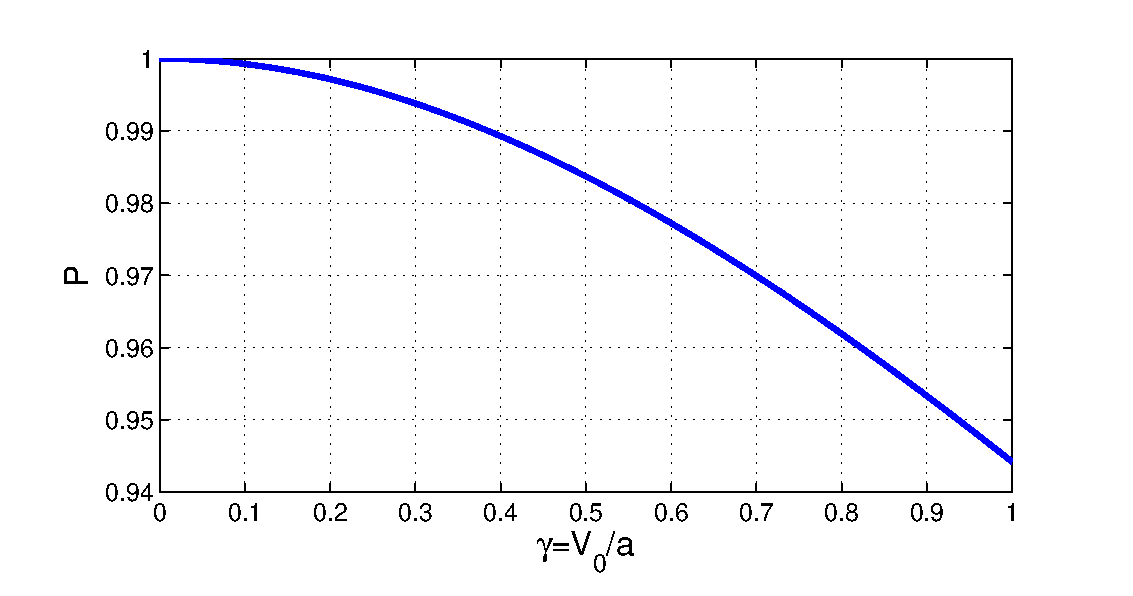
\includegraphics[scale=0.6]{P5_P.eps}
\caption {\small Exact probablity of  emaining in the ground state}
\label{P5-P}
\end{figure}

If we take a look at \eqref{P5-look} we can clearly see that both Hamiltonian are the same and we should just swap $\ket{1}$ & $\ket{2}$ that is those states should be mutually exchanged in our formulation If we reprsents the ground state of the new Hamiltonian as $\ket{\Omega_1}$ then from \eqref{P5-ground} we have:
\begin{equation}
c\ket{\Omega_1}=\left(1-\frac{2\gamma}{9}\right)\ket{2}+\left(1+\frac{\gamma}{9}\right)\ket{1}+\left(1+\frac{\gamma}{9}\right)\ket{3}
\end{equation} 
The probability for the electron to remain in the ground state is:
\begin{equation}
P=\abs{\bracket{\Omega_1}{\Phi_1}}^2\approx\left[\frac{2\left(1-\frac{2\gamma}{9}\right)\left(1+\frac{\gamma}{9}\right)+\left(1+\frac{\gamma}{9}\right)^2}{\left(1-\frac{2\gamma}{9}\right)^2+\left(1+\frac{\gamma}{9}\right)^2+\left(1+\frac{\gamma}{9}\right)^2}
\right]^2
\end{equation}


\end{homeworkSection}

\end{homeworkProblem}

